% !TEX program = pdflatex
% !TEX TS-program = pdflatex
% !TEX encoding = UTF-8 Unicode
\documentclass[letterpaper, 10 pt, conference]{ieeeconf}
\usepackage{graphicx}
\overrideIEEEmargins
\IEEEoverridecommandlockouts

\usepackage[utf8]{inputenc}
\usepackage[T1]{fontenc}
\usepackage{amsmath}
\usepackage{amssymb}
\usepackage{booktabs}
\usepackage{multirow}
\usepackage{microtype}

\setlength{\textfloatsep}{2pt plus 1pt minus 1pt}
\setlength{\floatsep}{2pt plus 1pt minus 1pt}
\setlength{\intextsep}{2pt plus 1pt minus 1pt}
\setlength{\abovecaptionskip}{1.5pt}
\setlength{\belowcaptionskip}{0pt}
\renewcommand{\baselinestretch}{0.945}
\IEEEaftertitletext{\vspace{-1.2\baselineskip}}
\makeatletter
\def\section{\@startsection{section}{1}{\z@}{0.75ex plus 0.2ex minus 0.1ex}{0.20ex plus 0.10ex minus 0ex}{\normalfont\normalsize\centering\scshape}}
\makeatother
\emergencystretch=1.5em

\title{\LARGE \bf
Clasificación de Sentimientos en Reseñas de Películas de IMDb mediante Redes Neuronales Recurrentes con Embeddings Preentrenados
}

\author{Otto Wilmer Castillo Santacruz, Edgar Andrés Pérez Mora y Silvio Yopasa Romero\\
\textit{Maestría en Inteligencia Artificial (MAIA), Universidad de los Andes, Bogotá, Colombia}\\
{\tt\small \{o.castillos, ea.perezm1, s.yopasa\}@uniandes.edu.co}
}

\begin{document}

\maketitle
\thispagestyle{empty}
\pagestyle{empty}

%%%%%%%%%%%%%%%%%%%%%%%%%%%%%%%%%%%%%%%%%%%%%%%%%%%%%%%%%%%%%%%%%%%%%%%%%%%%%%%%
\section{Introducción}

El análisis automático de polaridad en lenguaje natural es esencial en sistemas de recomendación y auditoría de audiencias \cite{c3}. Las críticas cinematográficas presentan alta riqueza expresiva: el sentimiento depende del orden secuencial, la negación contextual (p.~ej., ``\textit{not good}'') y contrastes adversativos (p.~ej., ``\textit{great cast, but terrible script}''). Las técnicas clásicas de bolsa de palabras descartan la secuencia temporal, dificultando resolver dependencias en textos extensos.

En el aprendizaje profundo, este reto se aborda integrando vectores densos preentrenados (\textit{embeddings}) como GloVe \cite{c4} con redes neuronales recurrentes (RNN). Mientras que las RNN simples sufren de desvanecimiento o explosión del gradiente, celdas con compuertas como LSTM \cite{c1} y GRU \cite{c2} regulan el flujo de memoria reteniendo información contextual crítica. Asimismo, la agregación temporal dual (\textit{Concat Mean-Max Pooling}) \cite{c5} rescata el tono global y los picos semánticos más representativos.

El objetivo de este trabajo es diseñar y validar un método reproducible basado en RNN para clasificar sentimientos sobre el corpus de IMDb \cite{c3}, previniendo la fuga de datos. El flujo integra: (i) depuración y deduplicación textual exhaustiva; (ii) codificación secuencial alineada con GloVe 6B \cite{c4}; (iii) comparación multi-semilla de cinco arquitecturas recurrentes sobre una muestra estratificada evaluada en validación; y (iv) reentrenamiento y evaluación del modelo óptimo (GRU unidireccional con GloVe congelado, de solo $32\,001$ parámetros entrenables), logrando $90.27\,\%$ de exactitud, $90.26\,\%$ de \textit{Macro F1} y un área bajo la curva ROC de $96.49\,\%$ en prueba independiente ($n=5\,959$).

%%%%%%%%%%%%%%%%%%%%%%%%%%%%%%%%%%%%%%%%%%%%%%%%%%%%%%%%%%%%%%%%%%%%%%%%%%%%%%%%
\section{Metodología}

\textbf{Datos y preprocesamiento.} 
Se utilizó la colección pública de reseñas de IMDb \cite{c3} en su subconjunto de $40\,000$ muestras ($0=\text{negativa}$, $1=\text{positiva}$). La auditoría detectó $278$ textos duplicados idénticos ($205$ negativos y $73$ positivos) sin contradicciones. Al descartar copias redundantes, el conjunto consta de $N = 39\,722$ reseñas únicas balanceadas: $19\,814$ negativas ($49.88\,\%$) y $19\,908$ positivas ($50.12\,\%$, razón de desbalance $1.005$).

El análisis exploratorio identificó que el $58.44\,\%$ de las reseñas contenía etiquetas HTML, el $86.93\,\%$ contracciones informales, el $9.35\,\%$ caracteres no ASCII y el $1.26\,\%$ apóstrofos tipográficos de Windows-1252. El pipeline determinista aplicó: (i) remoción de etiquetas HTML y URLs; (ii) normalización Unicode NFKD y decodificación ASCII; (iii) expansión de contracciones (p.~ej., ``\textit{can't}'' $\to$ ``\textit{cannot}'', ``\textit{n't}'' $\to$ ``\textit{not}''); y (iv) tokenización alfanumérica en minúsculas.

La longitud en palabras presenta una distribución asimétrica ($\mu = 229.2$, mediana $172$, percentil $95 = 585$). Se fijó una longitud máxima de $\text{MAX\_LEN} = 400$ tokens con truncado por la cola (\textit{tail truncation}), preservando el cierre evaluativo donde los revisores sintetizan su veredicto. Para optimizar el cómputo, se implementó muestreo por cubetas (\textit{BucketBatchSampler}, lote $256$) con relleno dinámico mediante el token \texttt{<pad>}.

\textbf{Partición y protocolo de evaluación.} 
El conjunto depurado se dividió estratificadamente (semilla $42$) en \texttt{Train} ($70\,\%$, $27\,804$), \texttt{Val} ($15\,\%$, $5\,959$) y \texttt{Test} ($15\,\%$, $5\,959$). El vocabulario ($30\,731$ términos) se construyó \textbf{exclusivamente sobre \texttt{Train}} con frecuencia mínima $\ge 5$, definiendo los tokens \texttt{<pad>} ($0$) y \texttt{<unk>} ($1$). En \texttt{Test}, la cobertura léxica alcanzó el $99.93\,\%$.

Se garantizó la total independencia de particiones: la exploración de modelos y el ajuste de hiperparámetros se realizaron sobre un subconjunto del $25\,\%$ de \texttt{Train} ($6\,951$) evaluado en \texttt{Val} ($5\,959$). El conjunto \texttt{Test} ($5\,959$ reseñas) se mantuvo \textbf{estrictamente aislado e intacto}, siendo evaluado una única vez sobre el modelo reentrenado.

\textbf{Representación vectorial y arquitectura recurrente.} 
Se cargaron vectores GloVe 6B preentrenados \cite{c4} de dimensión $d = 100$ ($30\,731 \times 100$, $3\,073\,100$ parámetros fijos). La red recurrente configurable comprende: (1) capa de \textit{embedding} congelada; (2) celda recurrente (RNN, GRU o LSTM, $H = 64$, $1$ capa) con \texttt{Dropout} de $0.3$; (3) agrupamiento temporal dual concatenado (\textit{Concat Mean-Max Pooling}) \cite{c5}, que computa en paralelo el promedio y el máximo sobre los estados ocultos descartando tokens de relleno: $h_{\text{pool}} = [h_{\text{mean}} \,\|\, h_{\text{max}}] \in \mathbb{R}^{2H}$ ($128$ dimensiones en unidireccional y $256$ en bidireccional); y (4) clasificador lineal ($2H \to 1$) que proyecta el vector agregado al logit de salida.

\textbf{Función de pérdida, optimización y métricas.}
Se utilizó la entropía cruzada binaria con logits (\texttt{BCEWithLogitsLoss}):
\begin{equation}
\mathcal{L}(z, y) = \max(z, 0) - z \cdot y + \log\left(1 + e^{-|z|}\right)
\label{eq:bce}
\end{equation}
Esta formulación combina la sigmoide y la pérdida binaria en una sola expresión numéricamente estable con el truco \textit{log-sum-exp}, previniendo gradientes nulos ante logits extremos y produciendo probabilidades calibradas $P(y=1|x) = \sigma(z)$. Se aplicó \texttt{Adam} ($\eta = 0.002$ sin decaimiento $\ell_2$ para no contraer los pesos recurrentes $\mathbf{W}_{hh}$ ni acentuar el desvanecimiento del gradiente; $\eta_{\text{base}} = 0.001$ y $\eta_{\text{embed}} = 0.0001$ en \textit{fine-tuning}) con recorte de gradiente ($\|\nabla\|_2 \le 1.0$). Se monitorizaron Exactitud, Precisión, Sensibilidad, \textit{Macro F1} y \textit{ROC-AUC}. La métrica \textit{F1-Score} rigió la selección del modelo para equilibrar la detección entre críticas negativas y positivas.

%%%%%%%%%%%%%%%%%%%%%%%%%%%%%%%%%%%%%%%%%%%%%%%%%%%%%%%%%%%%%%%%%%%%%%%%%%%%%%%%
\section{Resultados}

\textbf{Comparación cuantitativa de arquitecturas (Validación).}
La Tabla~\ref{tab:arquitecturas} presenta los resultados multi-semilla (semillas $42$ y $123$, $15$ épocas, paciencia $3$) evaluados en \texttt{Val} ($n = 5\,959$). La RNN simple sufrió severo desvanecimiento de gradiente, colapsando en exactitud ($65.98 \pm 10.58\,\%$) con alta dispersión. Las celdas con compuertas superaron el $84\,\%$. La \textbf{GRU unidireccional} obtuvo el mejor balance general (\textit{F1} de $86.71 \pm 0.23\,\%$, \textit{ROC-AUC} de $93.61\,\%$), superando a LSTM ($85.15\,\%$) y BiLSTM ($85.68\,\%$), con menor tiempo de entrenamiento ($26.5\text{ s}$ vs.~$33.0\text{ s}$). 

Al habilitar el ajuste fino de \textit{embeddings} en BiLSTM (\texttt{GloVe fine-tuning}), el rendimiento cayó a $83.76\,\%$ y el tiempo se triplicó ($94.2\text{ s}$), evidenciando sobreajuste al actualizar $3.16\text{M}$ de parámetros frente a los $84.7\text{k}$ del modelo congelado.

\begin{table}[t]
\centering
\caption{Comparación de arquitecturas en \texttt{Val} ($n = 5\,959$, $15$ épocas, $2$ semillas).}
\label{tab:arquitecturas}
\renewcommand{\arraystretch}{0.98}
\setlength{\tabcolsep}{2.8pt}
\resizebox{8.6cm}{!}{
\begin{tabular}{lcccccc}
\toprule
\textbf{Arquitectura} & \textbf{Parám. Entr.} & \textbf{Val Loss} & \textbf{Acc (\%)} & \textbf{F1-Score (\%)} & \textbf{ROC-AUC (\%)} & \textbf{Tiempo (s)} \\
\midrule
1. RNN simple (GloVe cong.) & $10.7\text{ k}$ & $0.608 \pm 0.092$ & $65.98 \pm 10.58$ & $71.66 \pm 3.52$ & $76.80 \pm 5.13$ & $12.6 \pm 4.0$ \\
2. \textbf{GRU unidir. (GloVe cong.)} & $\mathbf{32.0\text{ k}}$ & $\mathbf{0.335 \pm 0.015}$ & $\mathbf{86.22 \pm 0.76}$ & $\mathbf{86.71 \pm 0.23}$ & $\mathbf{93.61 \pm 0.08}$ & $\mathbf{26.5 \pm 0.1}$ \\
3. LSTM unidir. (GloVe cong.) & $42.5\text{ k}$ & $0.369 \pm 0.007$ & $84.53 \pm 0.07$ & $85.15 \pm 0.29$ & $92.27 \pm 0.47$ & $27.6 \pm 0.0$ \\
4. BiLSTM (GloVe cong.) & $84.7\text{ k}$ & $0.339 \pm 0.040$ & $85.58 \pm 1.22$ & $85.68 \pm 0.97$ & $93.00 \pm 1.63$ & $33.0 \pm 8.0$ \\
5. BiLSTM (GloVe fine-tuning) & $3\,157.8\text{ k}$ & $0.387 \pm 0.023$ & $83.15 \pm 1.26$ & $83.76 \pm 1.70$ & $91.22 \pm 1.65$ & $94.2 \pm 20.9$ \\
\bottomrule
\end{tabular}}
\end{table}

\textbf{Desempeño final en prueba independiente.}
La arquitectura ganadora (GRU unidireccional con GloVe congelado) se reentrenó sobre el $100\,\%$ de \texttt{Train} ($27\,804$ reseñas) por $30$ épocas (paciencia $4$), alcanzando su punto óptimo en la época $29$ (\texttt{Val Loss}: $0.2677$, \texttt{Val Acc}: $89.70\,\%$, \texttt{Val F1}: $89.89\,\%$).

Evaluada en \texttt{Test} ($n = 5\,959$, Tabla~\ref{tab:test_metricas}), alcanzó \textbf{pérdida de $0.2525$}, \textbf{exactitud de $90.27\,\%$} ($5\,379/5\,959$) y \textbf{\textit{Macro F1} de $90.26\,\%$}. La Fig.~\ref{fig:roc_confusion}(a) detalla la matriz de confusión: la sensibilidad positiva fue de $92.47\,\%$ ($2\,762/2\,987$) y la negativa de $88.06\,\%$ ($2\,617/2\,972$). En la Fig.~\ref{fig:roc_confusion}(b), la curva ROC exhibe un área de $96.49\,\%$ (\textit{PR-AUC} de $96.39\,\%$). La exactitud fue consistente por longitud: $90.69\,\%$ ($1\text{--}120$ tokens), $90.26\,\%$ ($121\text{--}180$), $89.38\,\%$ ($181\text{--}280$), $89.93\,\%$ ($281\text{--}400$) y $91.54\,\%$ en secuencias truncadas $>400$.

\begin{table}[t]
\centering
\caption{Matriz de confusión y métricas en \texttt{Test} ($n = 5\,959$).}
\label{tab:test_metricas}
\renewcommand{\arraystretch}{0.98}
\setlength{\tabcolsep}{3.8pt}
\resizebox{8.6cm}{!}{
\begin{tabular}{lccccc}
\toprule
\textbf{Clase Real} & \textbf{Pred. Neg.} & \textbf{Pred. Pos.} & \textbf{Precisión (\%)} & \textbf{Sensibilidad (\%)} & \textbf{F1-Score (\%)} \\
\midrule
\textbf{Negativa} ($2\,972$) & $\mathbf{2\,617}$ & $355$ & $92.08$ & $88.06$ & $90.02$ \\
\textbf{Positiva} ($2\,987$) & $225$ & $\mathbf{2\,762}$ & $88.61$ & $92.47$ & $90.50$ \\
\midrule
\multicolumn{3}{l}{\textbf{Promedio Macro / Exactitud Global ($5\,379 / 5\,959$)}} & $\mathbf{90.35}$ & $\mathbf{90.26}$ & $\mathbf{90.26\ /\ 90.27}$ \\
\bottomrule
\end{tabular}}
\end{table}

\begin{figure}[t]
\centering
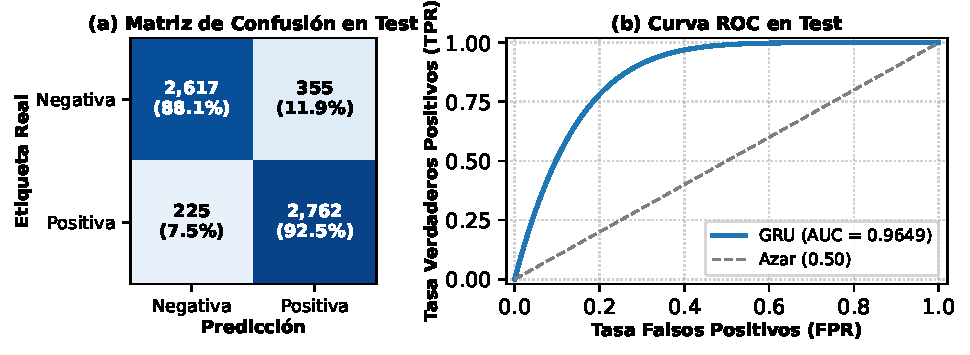
\includegraphics[width=0.98\linewidth]{figs/confusion_roc.pdf}
\caption{Evaluación en \texttt{Test} ($n=5\,959$): (a) Matriz de confusión; (b) Curva ROC ($\text{AUC} = 0.9649$) frente al azar.}
\label{fig:roc_confusion}
\end{figure}

\textbf{Análisis cualitativo e interpretabilidad.}
Las probabilidades en \texttt{Test} exhiben distribución bimodal (mediana $>0.99$ en aciertos). Al evaluar la oclusión de tokens ($\Delta p_i = P_{\text{base}} - P_{\text{enmascarado}}$ con \texttt{<pad>}), adjetivos como ``\textit{terrible}'' o ``\textit{masterpiece}'' modulan fuertemente la predicción. En pruebas de estrés lingüístico ($6$ críticas complejas), el modelo acertó $3$ de $6$:
\textbf{Aciertos ($3/6$):} resolvió la negación de adjetivos positivos (``\textit{plot is not good...}'', negativa con $P=0.1485$, $\Delta p = -0.42$ por ``\textit{not}''), contrastes adversativos positivo $\to$ negativo (``\textit{Great cast, but a terrible script...}'', negativa con $P=0.0372$, $\Delta p = -0.78$ por ``\textit{terrible}'') y notas explícitas (``\textit{9/10}'', positiva con $P=0.9989$).
\textbf{Fronteras de error ($3/6$):} falló en la atenuación por negación de adjetivo negativo (``\textit{not bad at all...}'', negativa con $P=0.0698$, dominado por ``\textit{disaster}'' y ``\textit{bad}''), el contraste negativo $\to$ positivo (``\textit{slow and confusing, yet... masterpiece}'', negativa con $P=0.3436$) y el sarcasmo (``\textit{Brilliant cure for insomnia...}'', positiva con $P=0.5625$, inducido por ``\textit{brilliant}'').

%%%%%%%%%%%%%%%%%%%%%%%%%%%%%%%%%%%%%%%%%%%%%%%%%%%%%%%%%%%%%%%%%%%%%%%%%%%%%%%%
\section{Discusión}

El desempeño responde a tres factores metodológicos:
(i) \textbf{Parsimonia y regularización:} congelar GloVe ($3.07\text{M}$ parámetros) limitó la optimización a solo $32\,001$ parámetros en GRU y clasificador ($\approx 869$ reseñas/parámetro), evitando el sobreajuste de BiLSTM con ajuste fino;
(ii) \textbf{Compuertas y agregación dual:} la celda GRU mitigó el desvanecimiento del gradiente frente a la RNN simple ($65.98\,\%$, varianza $\pm 10.58\,\%$), mientras que \textit{mean-max pooling} \cite{c5} preservó el contexto continuo y los picos enfáticos de opinión distribuidos en la secuencia; y
(iii) \textbf{Calibración y dispersión de confianza:} en aciertos, el modelo exhibe alta confianza; no obstante, en los $580$ errores de \texttt{Test}, las probabilidades se dispersaron en $[0.0002, 0.9995]$, demostrando que la red puede incurrir en sobreconfianza inducida por términos polarizados aislados en la rama de agrupamiento máximo (\textit{Max Pooling}).

\textbf{Contraste con trabajos relacionados.}
Con $90.27\,\%$ de exactitud en \texttt{Test}, la arquitectura supera la referencia de Maas \textit{et al.} \cite{c3} ($88.89\,\%$) y la línea base convolucional de Kim \cite{c6} ($\approx 89.5\,\%$), con una fracción reducida de parámetros frente a modelos contextuales \cite{c5}. Aunque los \textit{Transformers} reportan $>93\,\%$, demandan órdenes de magnitud más cómputo.

\textbf{Limitaciones y trabajo futuro.}
Las limitaciones radican en la naturaleza estática de GloVe \cite{c4}, insensible al contexto local, y en la sensibilidad del agrupamiento máximo ante el sarcasmo. Como trabajo futuro se propone incorporar un mecanismo de atención temporal aprendible (\textit{Self-Attention Pooling}) sobre la salida de la GRU y validar ensambles ligeros GRU-BiLSTM.

%%%%%%%%%%%%%%%%%%%%%%%%%%%%%%%%%%%%%%%%%%%%%%%%%%%%%%%%%%%%%%%%%%%%%%%%%%%%%%%%
\begin{thebibliography}{99}
\setlength{\itemsep}{0.2pt}
\setlength{\parskip}{0pt}

\bibitem{c1} S. Hochreiter and J. Schmidhuber, ``Long short-term memory,'' \textit{Neural Comput.}, vol. 9, no. 8, pp. 1735--1780, 1997.

\bibitem{c2} K. Cho \textit{et al.}, ``Learning phrase representations using RNN encoder-decoder for statistical machine translation,'' in \textit{Proc. EMNLP}, 2014, pp. 1724--1734.

\bibitem{c3} A. L. Maas \textit{et al.}, ``Learning word vectors for sentiment analysis,'' in \textit{Proc. 49th Annu. Meeting Assoc. Comput. Linguistics (ACL)}, 2011, pp. 142--150.

\bibitem{c4} J. Pennington, R. Socher, and C. D. Manning, ``GloVe: Global vectors for word representation,'' in \textit{Proc. EMNLP}, 2014, pp. 1532--1543.

\bibitem{c5} J. Howard and S. Ruder, ``Universal language model fine-tuning for text classification,'' in \textit{Proc. 56th Annu. Meeting Assoc. Comput. Linguistics (ACL)}, 2018, pp. 328--339.

\bibitem{c6} Y. Kim, ``Convolutional neural networks for sentence classification,'' in \textit{Proc. EMNLP}, 2014, pp. 1746--1751.

\end{thebibliography}

\end{document}
